\section{Experimentación y resultados}
\label{sec:experimentacion}

\subsection{Diseño experimental}

\begin{itemize}
  \item \textbf{Instancias.} Los dos hoteles, con $\Tmax = 480$ min y sin preferencias.
  \item \textbf{Presupuesto.} Todos los métodos estocásticos realizan exactamente 20.100 evaluaciones por ejecución. La heurística voraz es determinista.
  \item \textbf{Repeticiones.} 15 semillas independientes: 42, 101, 203, 314, 456, 578, 619, 723, 831, 954, 1024, 1234, 2048, 3072 y 4096.
  \item \textbf{Métricas.} Hipervolumen con punto de referencia $(\Tmax, 0) = (480\ \text{min}, 0\ \text{puntos})$ y \emph{spread} $\Delta$. Se informa de la media y de la desviación típica poblacional de las 15 ejecuciones.
  \item \textbf{Contraste.} Test pareado bilateral de rangos con signo de Wilcoxon sobre el hipervolumen de cada línea base frente a NSGA-II, con $\alpha = 0{,}05$.
\end{itemize}

\subsection{Validación en problemas de prueba}
\label{sec:zdt}

Antes de aplicarlo al caso real, el núcleo de NSGA-II (ordenación no dominada, aglomeración y torneo) se validó en tres problemas ZDT \citep{zitzler2000} con 30 variables continuas en $[0,1]$, cuyo frente es conocido. En los tres, $f_1(x) = x_1$, $g(x) = 1 + \frac{9}{29}\sum_{i=2}^{30} x_i$ y $f_2(x) = g(x)\,h(f_1, g)$, y el frente óptimo corresponde a $g(x) = 1$. Para variables continuas se usaron el cruce SBX ($\eta_c = 15$, cada variable cruzada con probabilidad 0,5) y la mutación polinomial ($\eta_m = 20$, probabilidad $1/30$ por variable), con $N = 100$, $G = 250$ y semilla 42.

\begin{table}[H]
\centering
\small
\caption{Validación de NSGA-II en la familia ZDT (IGD frente a 500 puntos del frente teórico).}
\label{tab:zdt}
\begin{tabular}{@{}l l l c c@{}}
\toprule
Problema & Frente & $h(f_1, g)$ & Soluciones & IGD \\
\midrule
ZDT1 & Convexo & $1 - \sqrt{f_1/g}$ & 100 & 0,0210 \\
ZDT2 & No convexo & $1 - (f_1/g)^2$ & 100 & 0,0547 \\
ZDT3 & Discontinuo & $1 - \sqrt{f_1/g} - (f_1/g)\sin(10\pi f_1)$ & 100 & 0,0127 \\
\bottomrule
\end{tabular}
\end{table}

\begin{figure}[H]
\centering
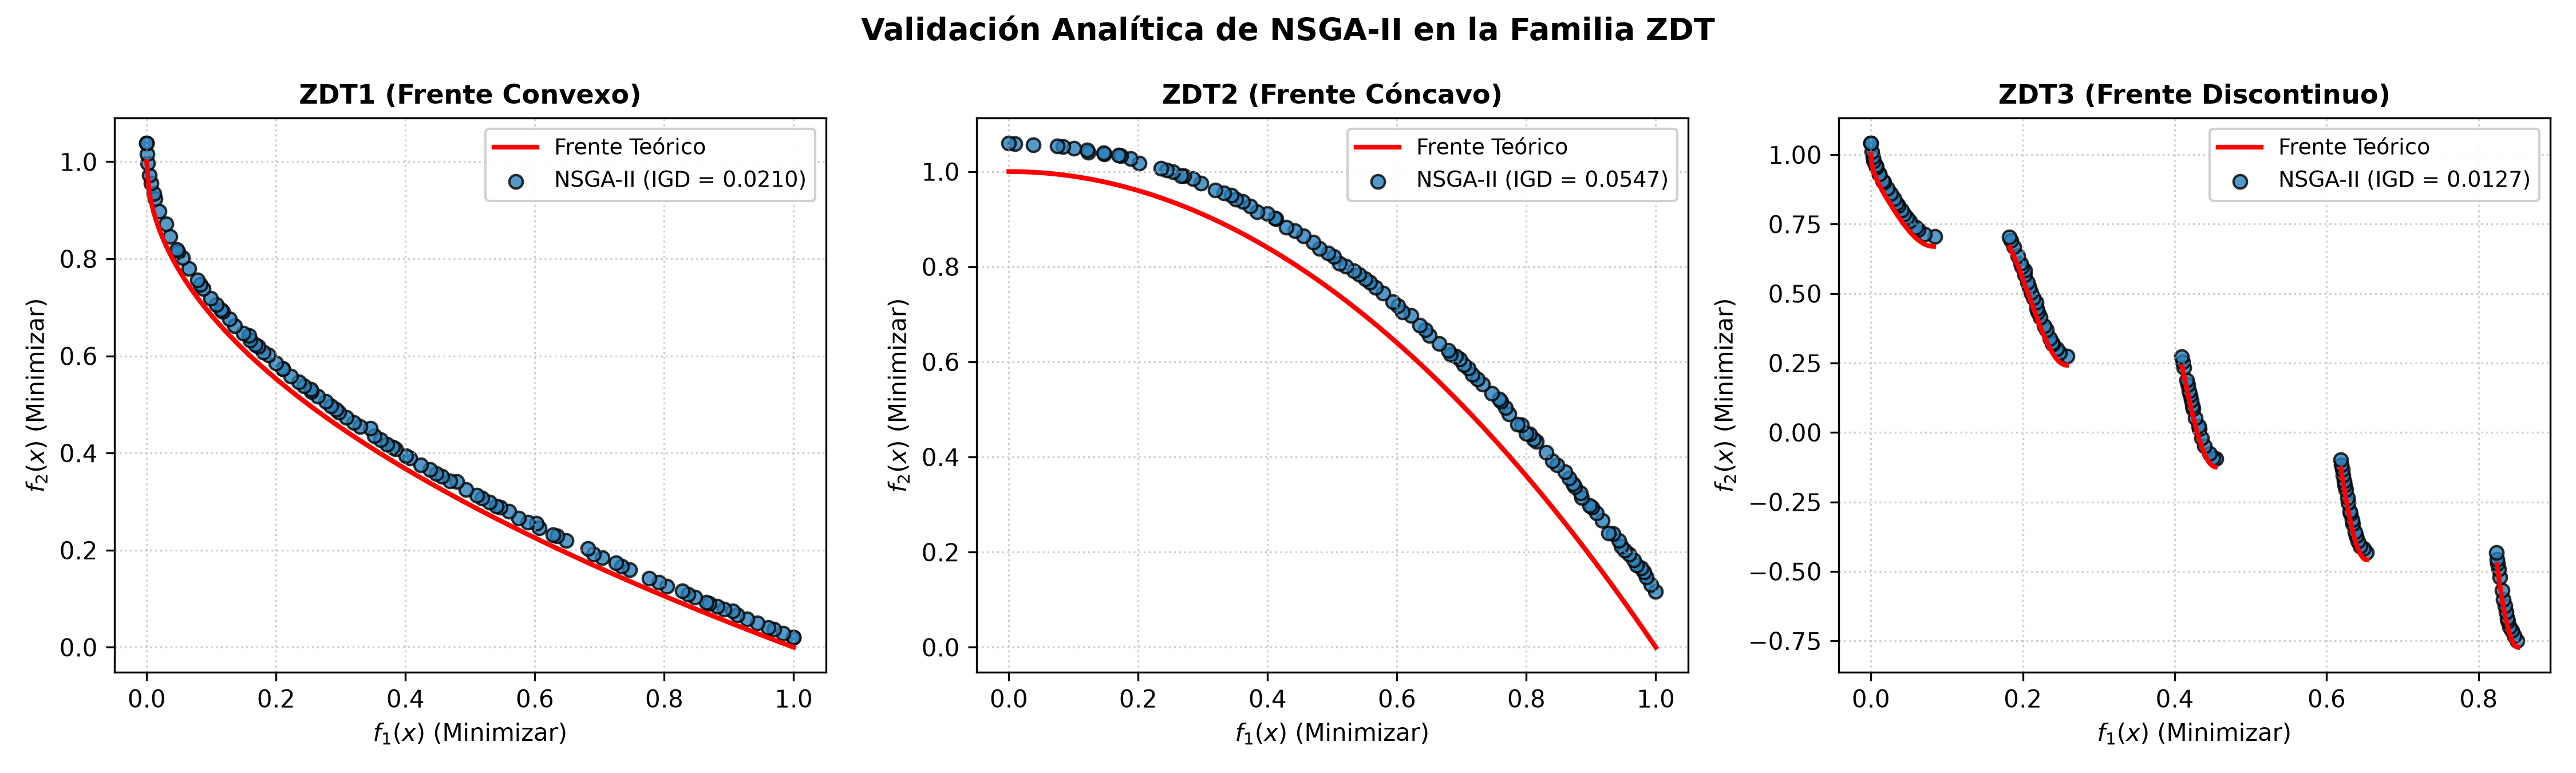
\includegraphics[width=\textwidth]{validacion_zdt_familia.png}
\caption{Frentes obtenidos por NSGA-II (puntos) frente a los frentes teóricos (línea) en ZDT1, ZDT2 y ZDT3.}
\label{fig:zdt}
\end{figure}

En los tres casos las 100 soluciones cubren todo el rango de $f_1$. En ZDT3 el algoritmo encuentra los cinco tramos del frente discontinuo y en ZDT1 queda muy cerca del frente. En ZDT2, de frente no convexo, la cobertura es completa pero las soluciones quedan algo por encima del frente teórico (figura~\ref{fig:zdt}), lo que explica su mayor IGD: con 250 generaciones la convergencia en ese problema todavía no es completa. La validación confirma que los mecanismos de dominancia y de diversidad funcionan en frentes convexos, no convexos y discontinuos.

\subsection{Comparación de algoritmos en Gran Canaria}

La tabla~\ref{tab:resultados} recoge los resultados de las 15 semillas y la figura~\ref{fig:boxplot}, su distribución.

\begin{table}[H]
\centering
\small
\caption{Hipervolumen (media $\pm$ desviación típica, 15 semillas), \emph{spread} medio y test de Wilcoxon frente a NSGA-II. La mejora es la de NSGA-II sobre cada método.}
\label{tab:resultados}
\begin{tabular}{@{}l r c c r@{}}
\toprule
Algoritmo & Hipervolumen & $\Delta$ & $p$ vs NSGA-II & Mejora \\
\midrule
\multicolumn{5}{@{}l}{\emph{Hotel Santa Catalina (Las Palmas)}} \\
NSGA-II & \textbf{11.594,3 $\pm$ 24,5} & 0,428 & --- & --- \\
Voraz & 10.188,9 $\pm$ 0,0 & 0,275 & $6{,}4 \times 10^{-4}$ & +13,8 \% \\
Búsqueda aleatoria & 10.050,3 $\pm$ 99,9 & 0,447 & $6{,}1 \times 10^{-5}$ & +15,4 \% \\
$\varepsilon$-restricción & 9.711,9 $\pm$ 254,0 & 0,307 & $6{,}1 \times 10^{-5}$ & +19,4 \% \\
Suma ponderada & 6.839,8 $\pm$ 490,3 & 1,076 & $6{,}1 \times 10^{-5}$ & +69,5 \% \\
\midrule
\multicolumn{5}{@{}l}{\emph{Hotel Lopesan Villa del Conde (Meloneras)}} \\
NSGA-II & \textbf{10.013,1 $\pm$ 64,4} & 0,597 & --- & --- \\
Voraz & 9.095,0 $\pm$ 0,0 & 0,346 & $6{,}1 \times 10^{-5}$ & +10,1 \% \\
Búsqueda aleatoria & 8.694,5 $\pm$ 90,4 & 0,632 & $6{,}1 \times 10^{-5}$ & +15,2 \% \\
$\varepsilon$-restricción & 8.389,8 $\pm$ 286,4 & 0,332 & $6{,}1 \times 10^{-5}$ & +19,3 \% \\
Suma ponderada & 5.411,4 $\pm$ 726,3 & 1,091 & $6{,}1 \times 10^{-5}$ & +85,0 \% \\
\bottomrule
\end{tabular}
\end{table}

\begin{figure}[H]
\centering
\begin{subfigure}{0.49\textwidth}
  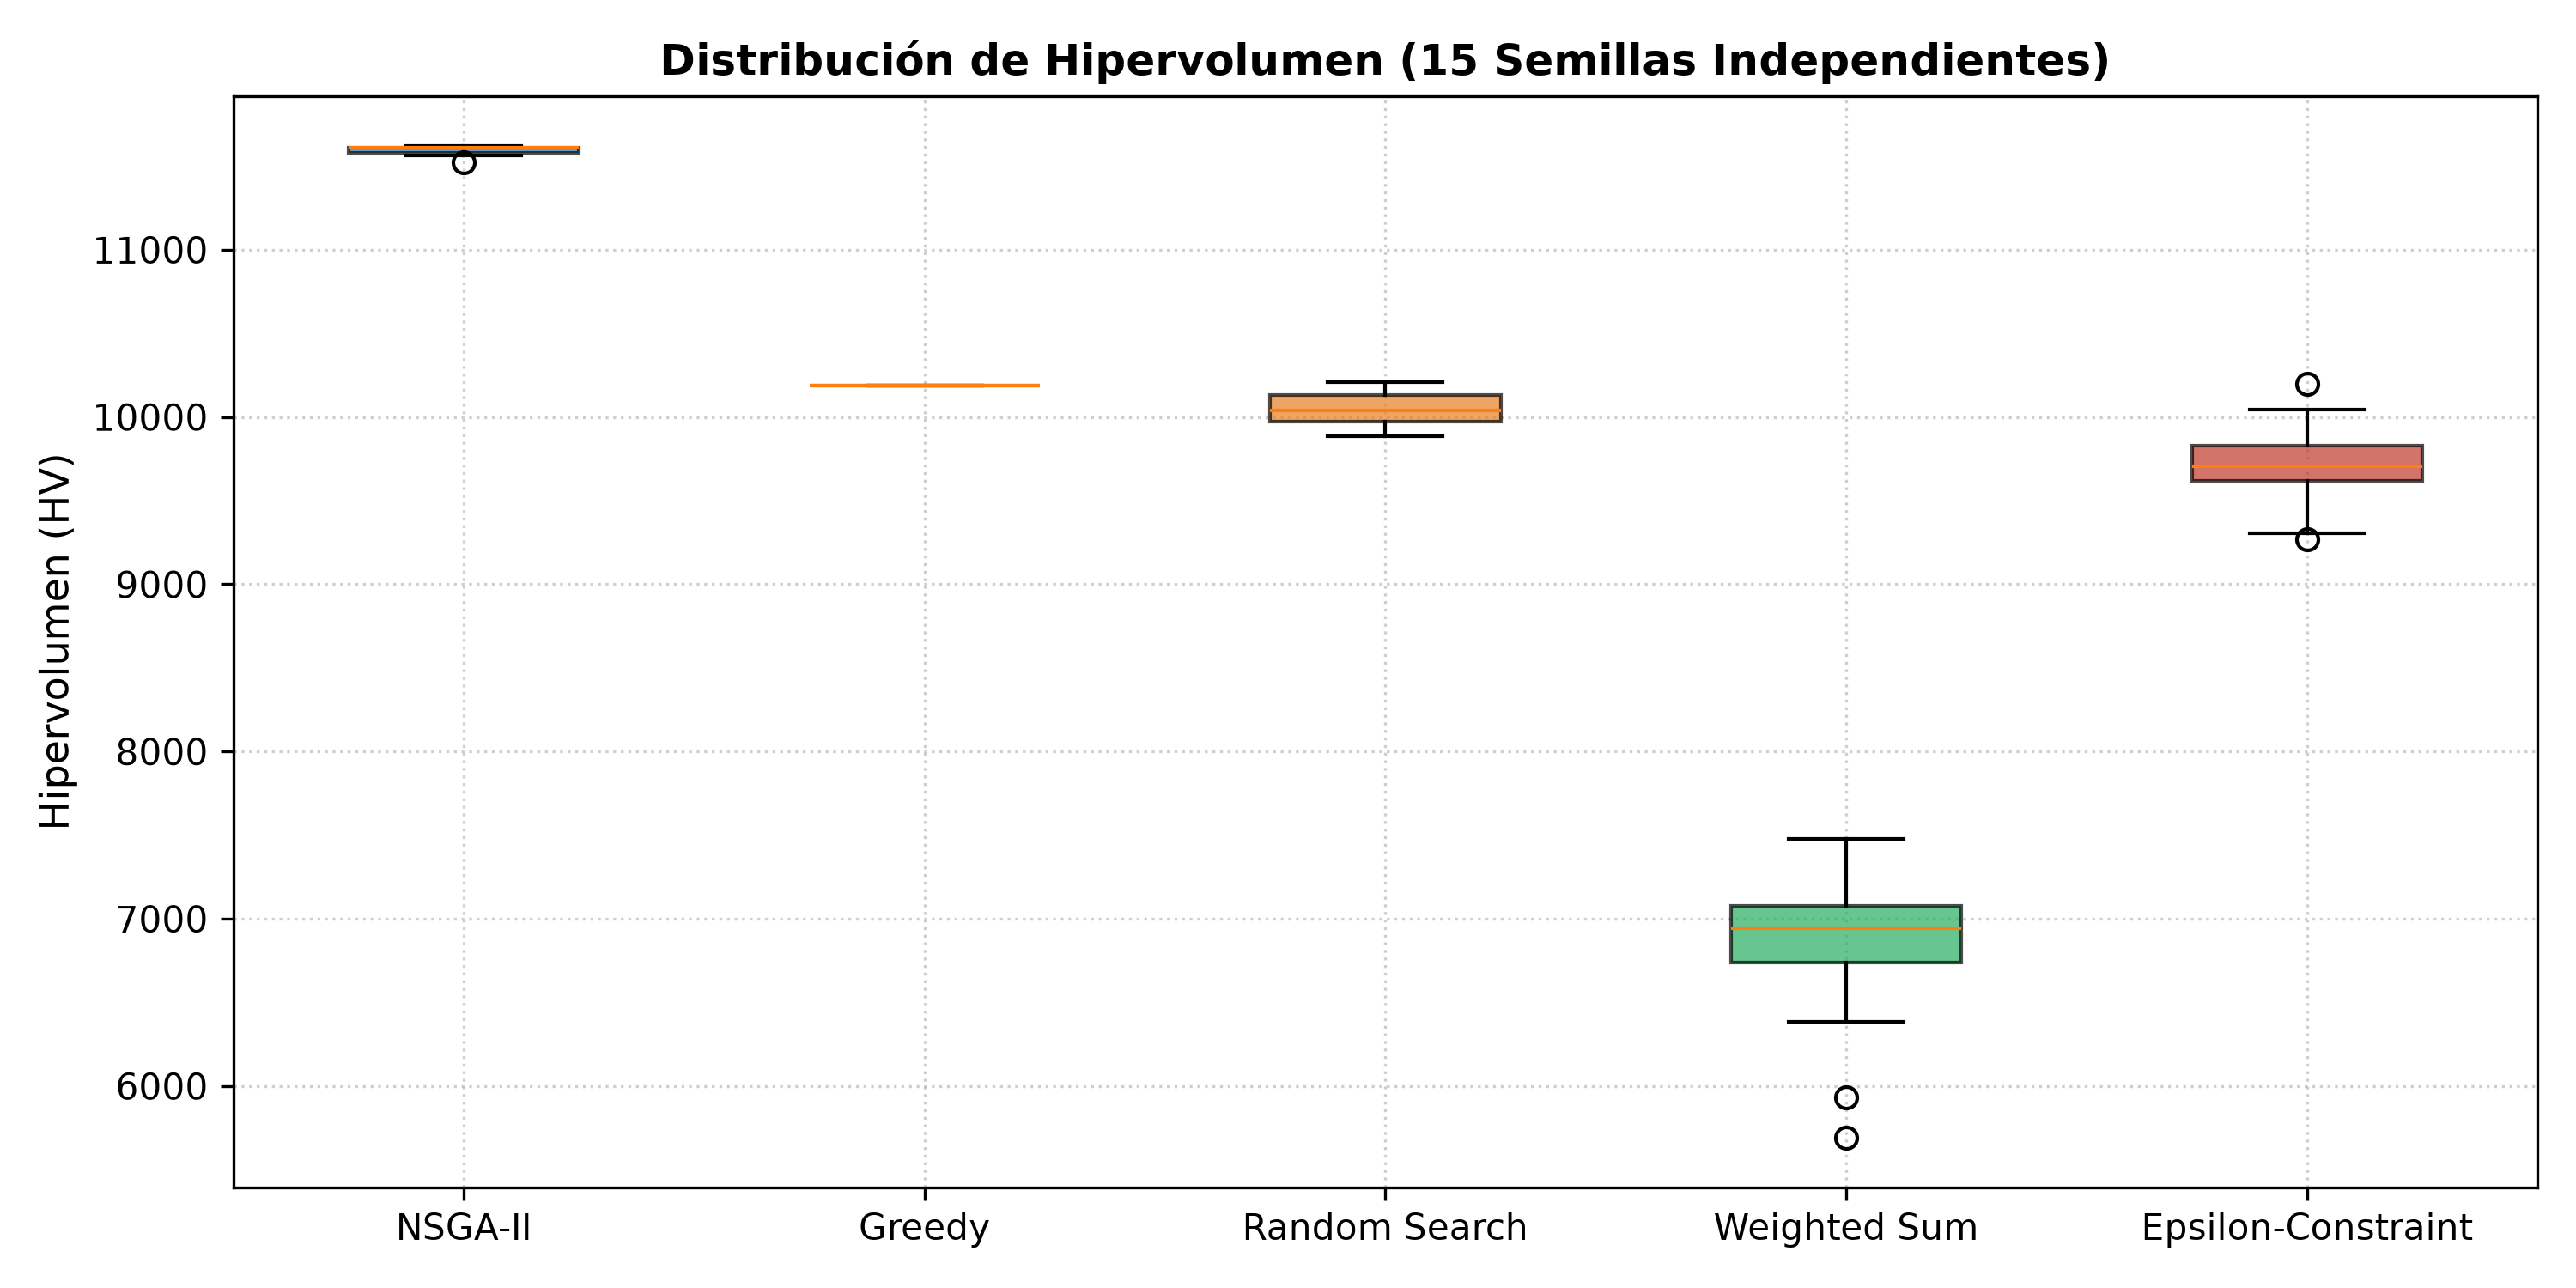
\includegraphics[width=\textwidth]{santa_catalina/boxplot_hipervolumen.png}
  \caption{Santa Catalina}
\end{subfigure}\hfill
\begin{subfigure}{0.49\textwidth}
  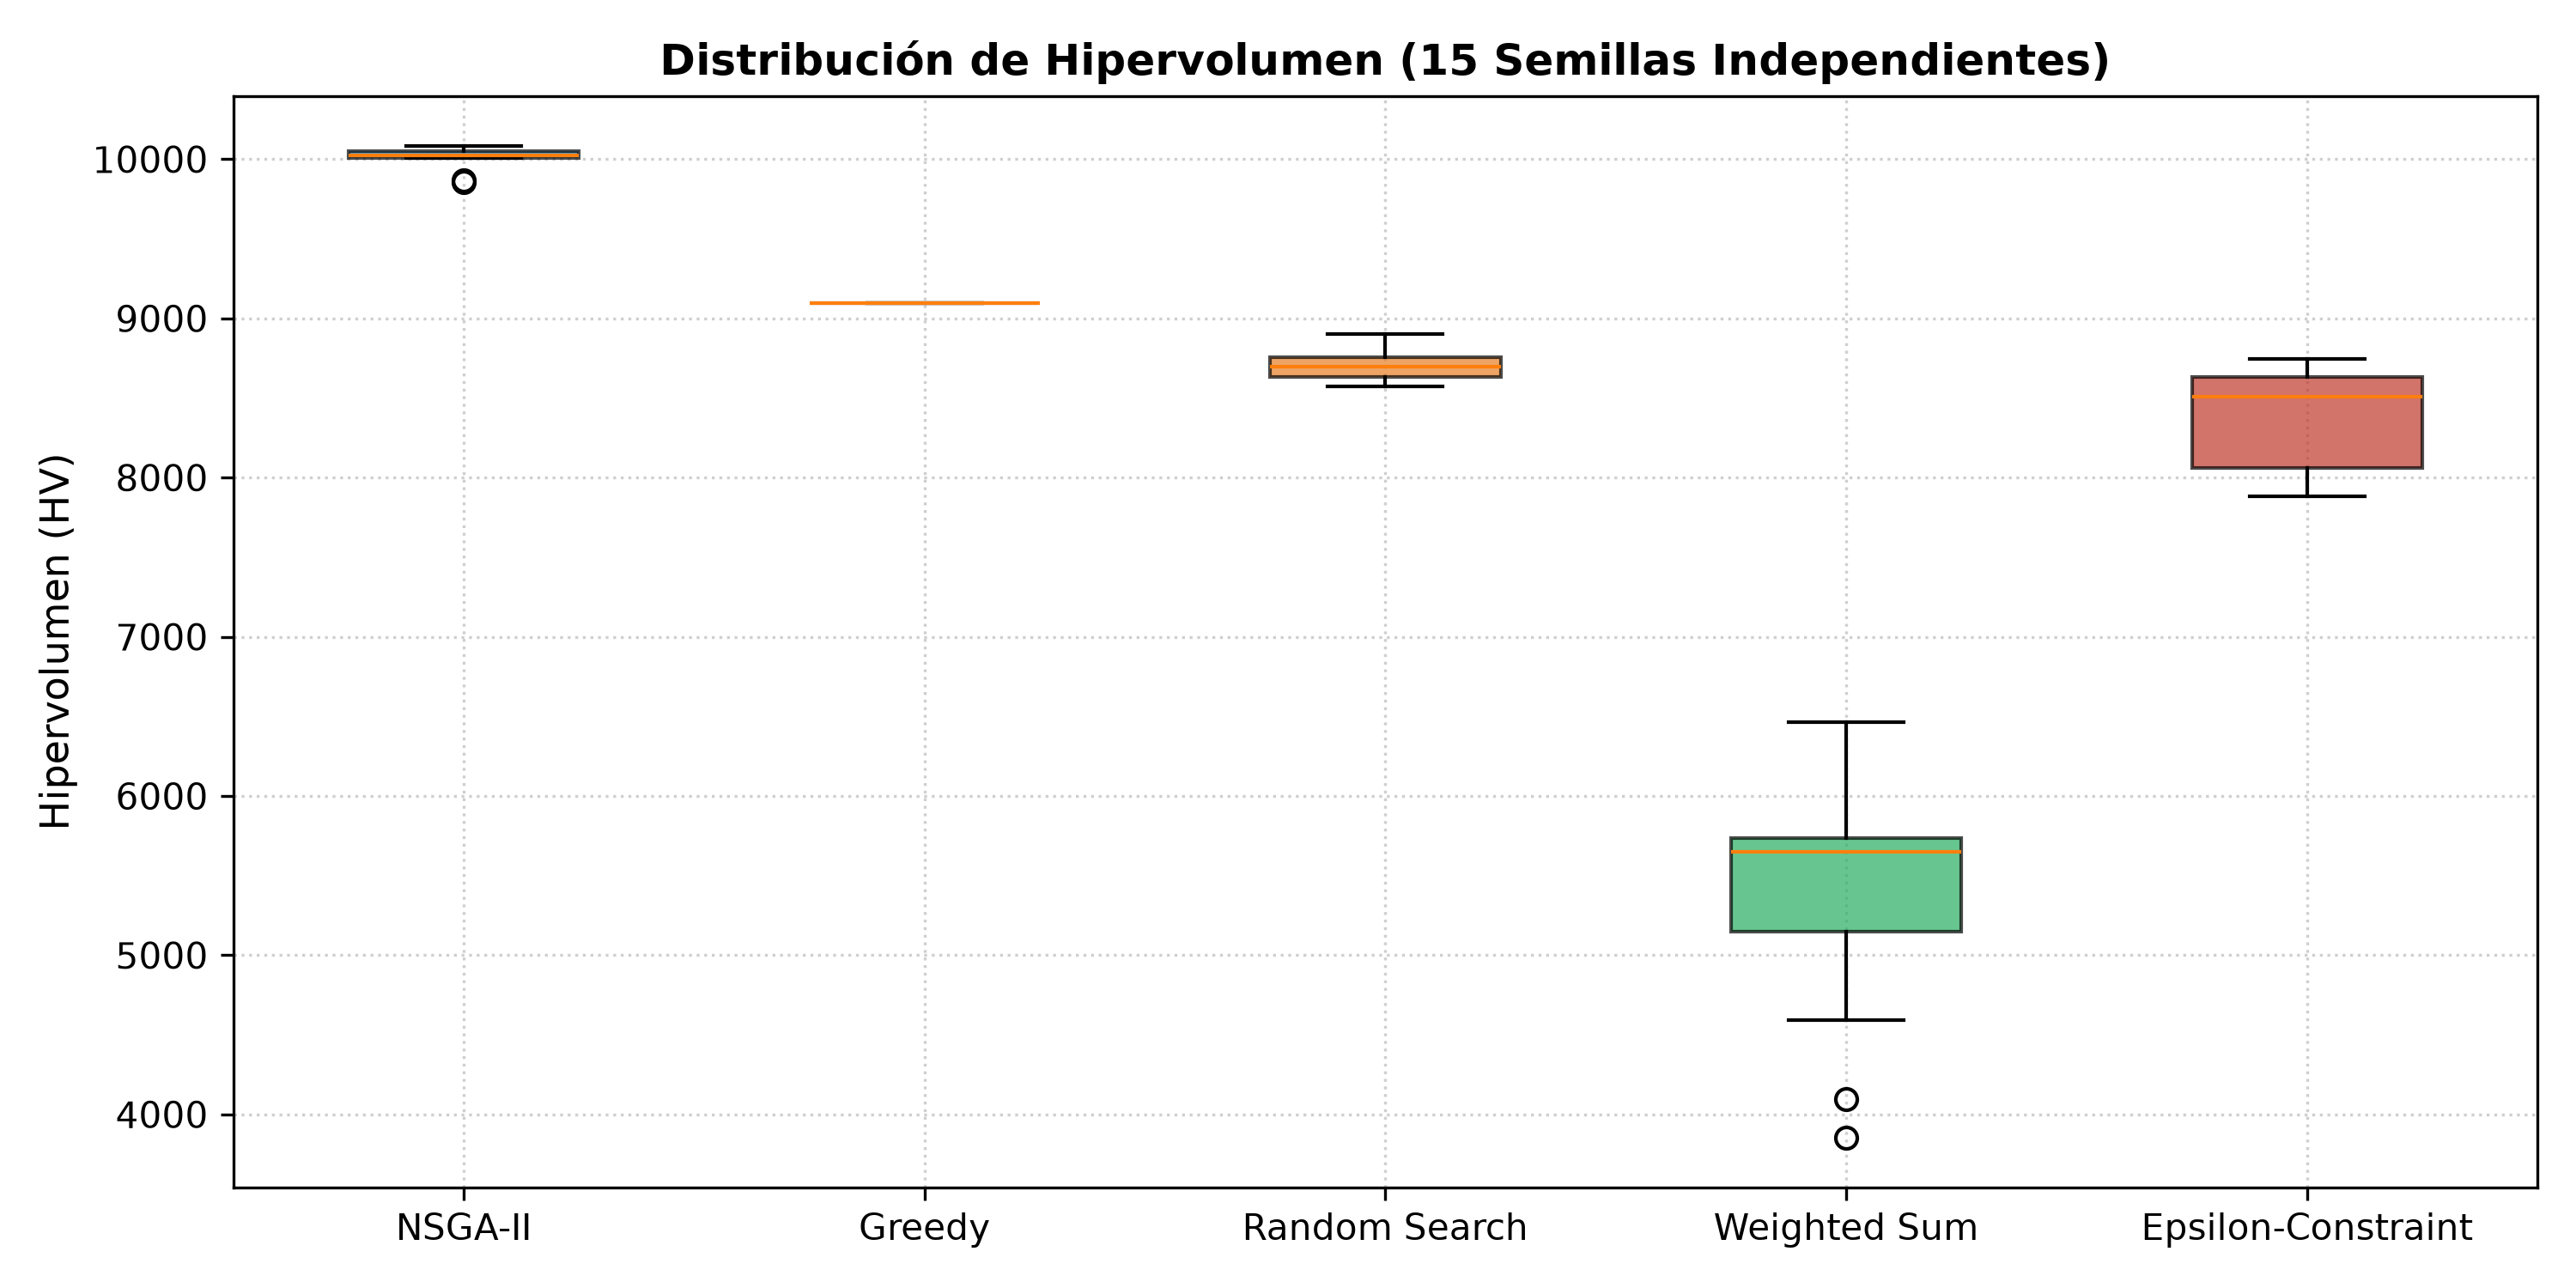
\includegraphics[width=\textwidth]{lopesan_villa_del_conde/boxplot_hipervolumen.png}
  \caption{Lopesan Villa del Conde}
\end{subfigure}
\caption{Distribución del hipervolumen de cada algoritmo en las 15 semillas.}
\label{fig:boxplot}
\end{figure}

NSGA-II obtiene el mayor hipervolumen en los dos hoteles, con diferencias significativas frente a las cuatro líneas base ($p < 0{,}001$). Gana además en las 15 semillas: su peor ejecución (11.524,5 en Santa Catalina y 9.857,0 en Lopesan) supera a la mejor de cualquier otro método. El valor $6{,}1 \times 10^{-5} = 2/2^{15}$ es el menor $p$-valor posible del test exacto de Wilcoxon con 15 pares. Frente a la heurística voraz en Santa Catalina, varias semillas de NSGA-II dan el mismo hipervolumen y la voraz es constante, así que hay empates en las diferencias y SciPy usa la aproximación normal ($p = 6{,}4 \times 10^{-4}$). La desviación típica de NSGA-II es pequeña: un 0,2 \% de la media en Santa Catalina y un 0,6 \% en Lopesan.

\paragraph{Convergencia.} La figura~\ref{fig:convergencia} muestra la evolución de una ejecución. El hipervolumen supera al de la heurística voraz en torno a la generación 10, alcanza el 99 \% de su valor final en la generación 139 y sigue mejorando despacio hasta la 200. La mejor puntuación factible avanza a saltos, cuando el algoritmo encuentra una combinación nueva de POIs que cabe en las 8 horas.

\begin{figure}[H]
\centering
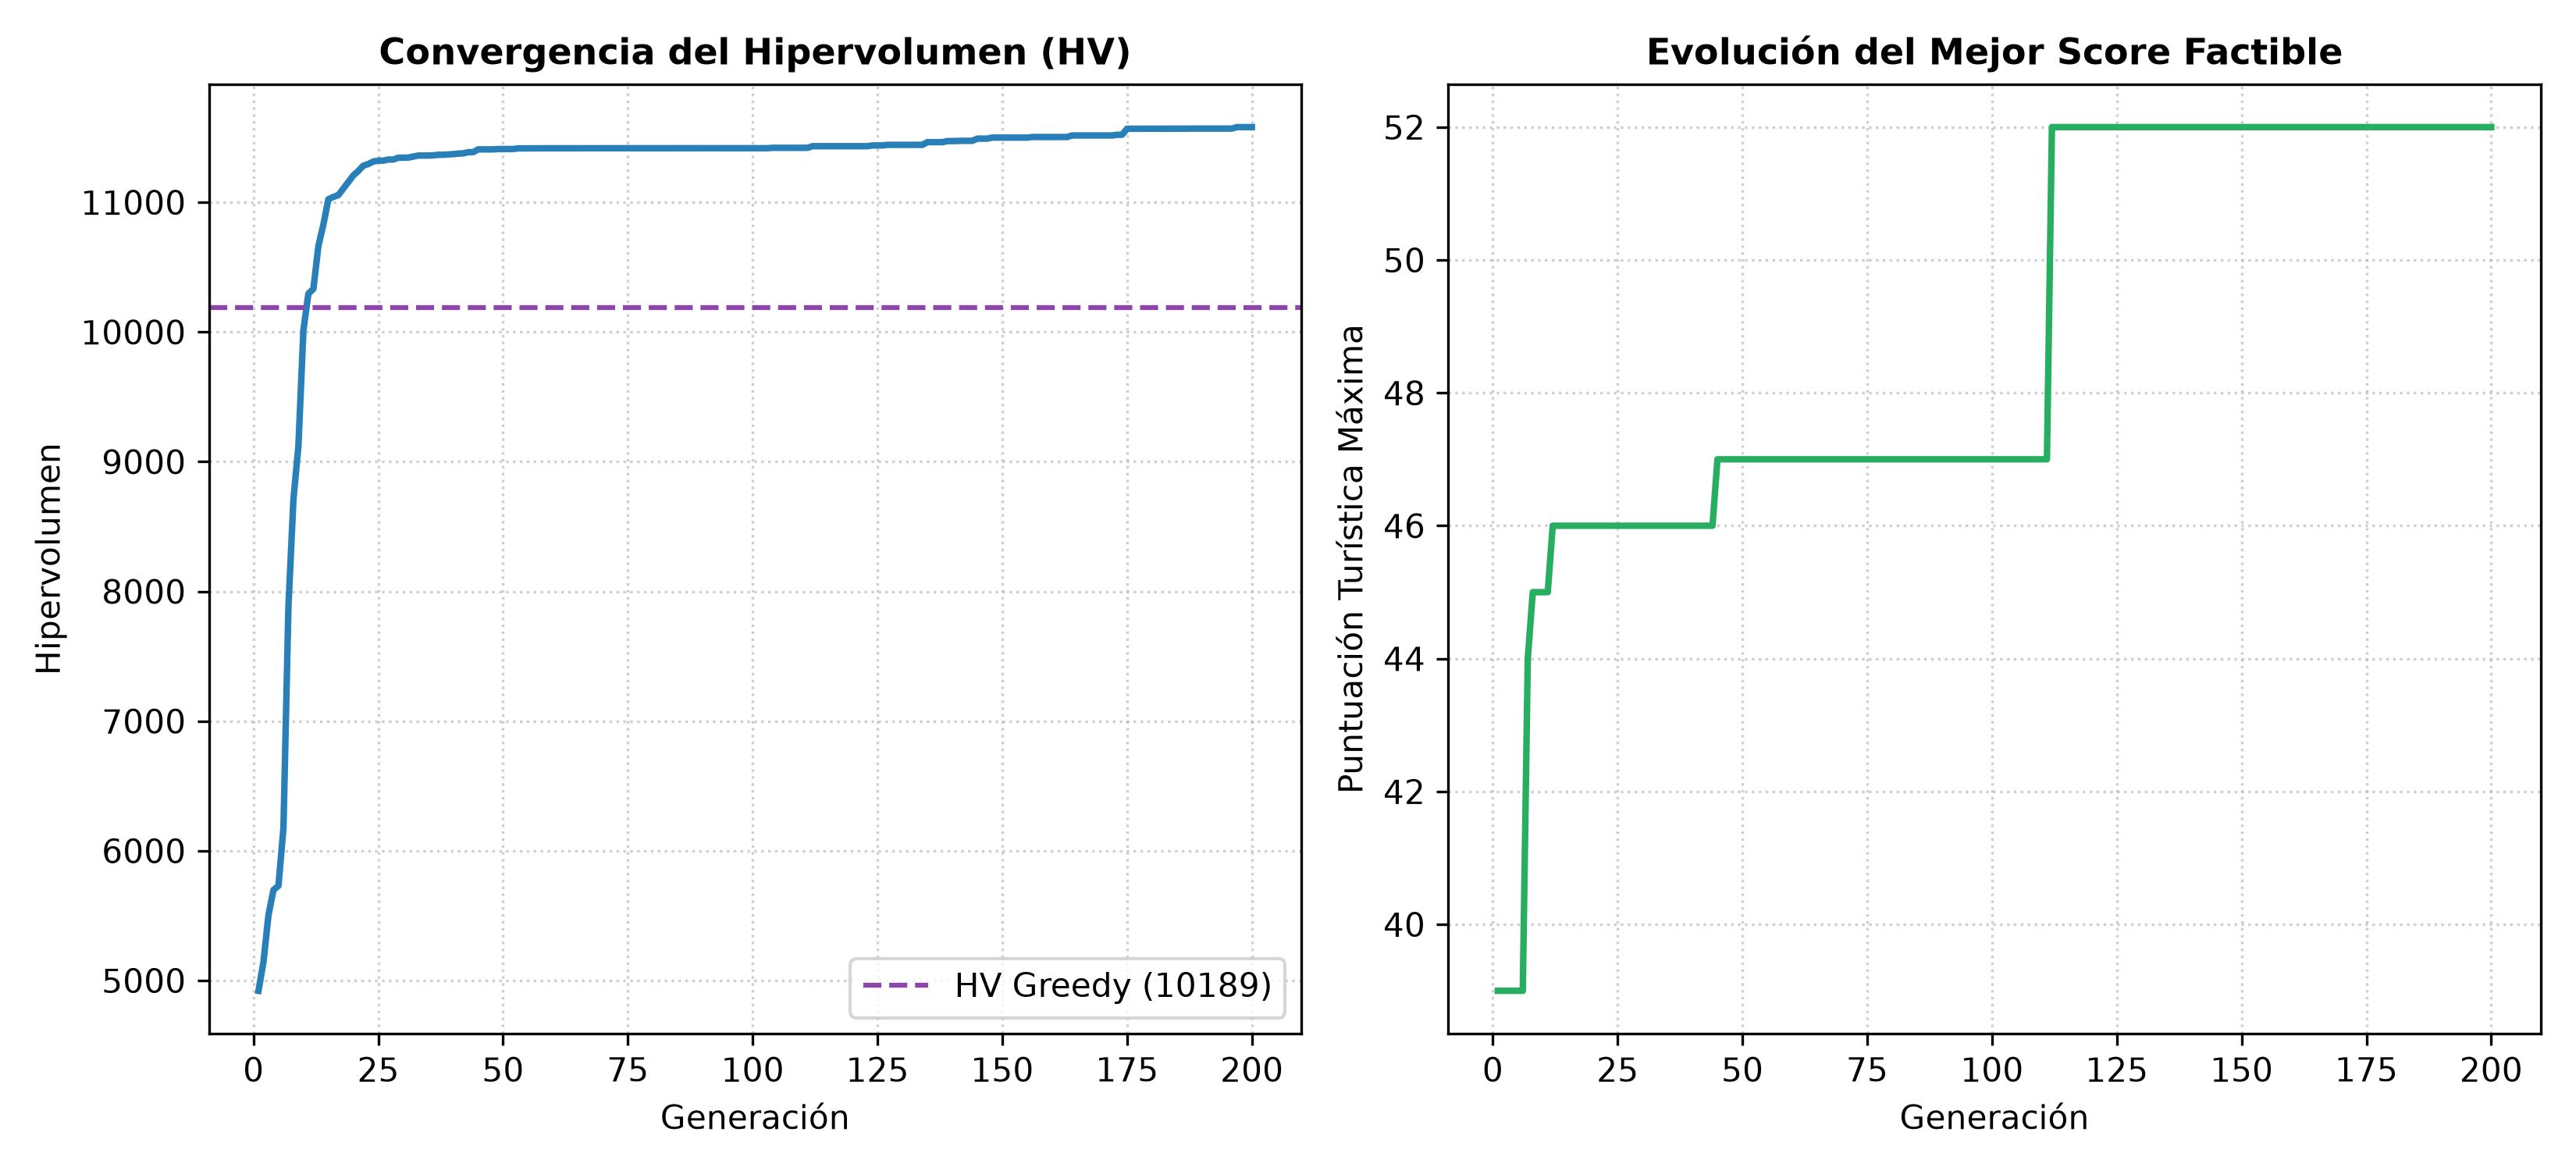
\includegraphics[width=0.9\textwidth]{santa_catalina/convergencia_nsga2.png}
\caption{Convergencia de NSGA-II en Santa Catalina (semilla 42): hipervolumen y mejor puntuación factible por generación. La línea discontinua es el hipervolumen de la heurística voraz.}
\label{fig:convergencia}
\end{figure}

\subsection{Frentes de Pareto y rutas recomendadas}

La figura~\ref{fig:frentes} muestra el frente de cada hotel con la semilla 42 y la tabla~\ref{tab:rutas}, las tres rutas recomendadas (sección~\ref{sec:recomendadas}).

\begin{figure}[H]
\centering
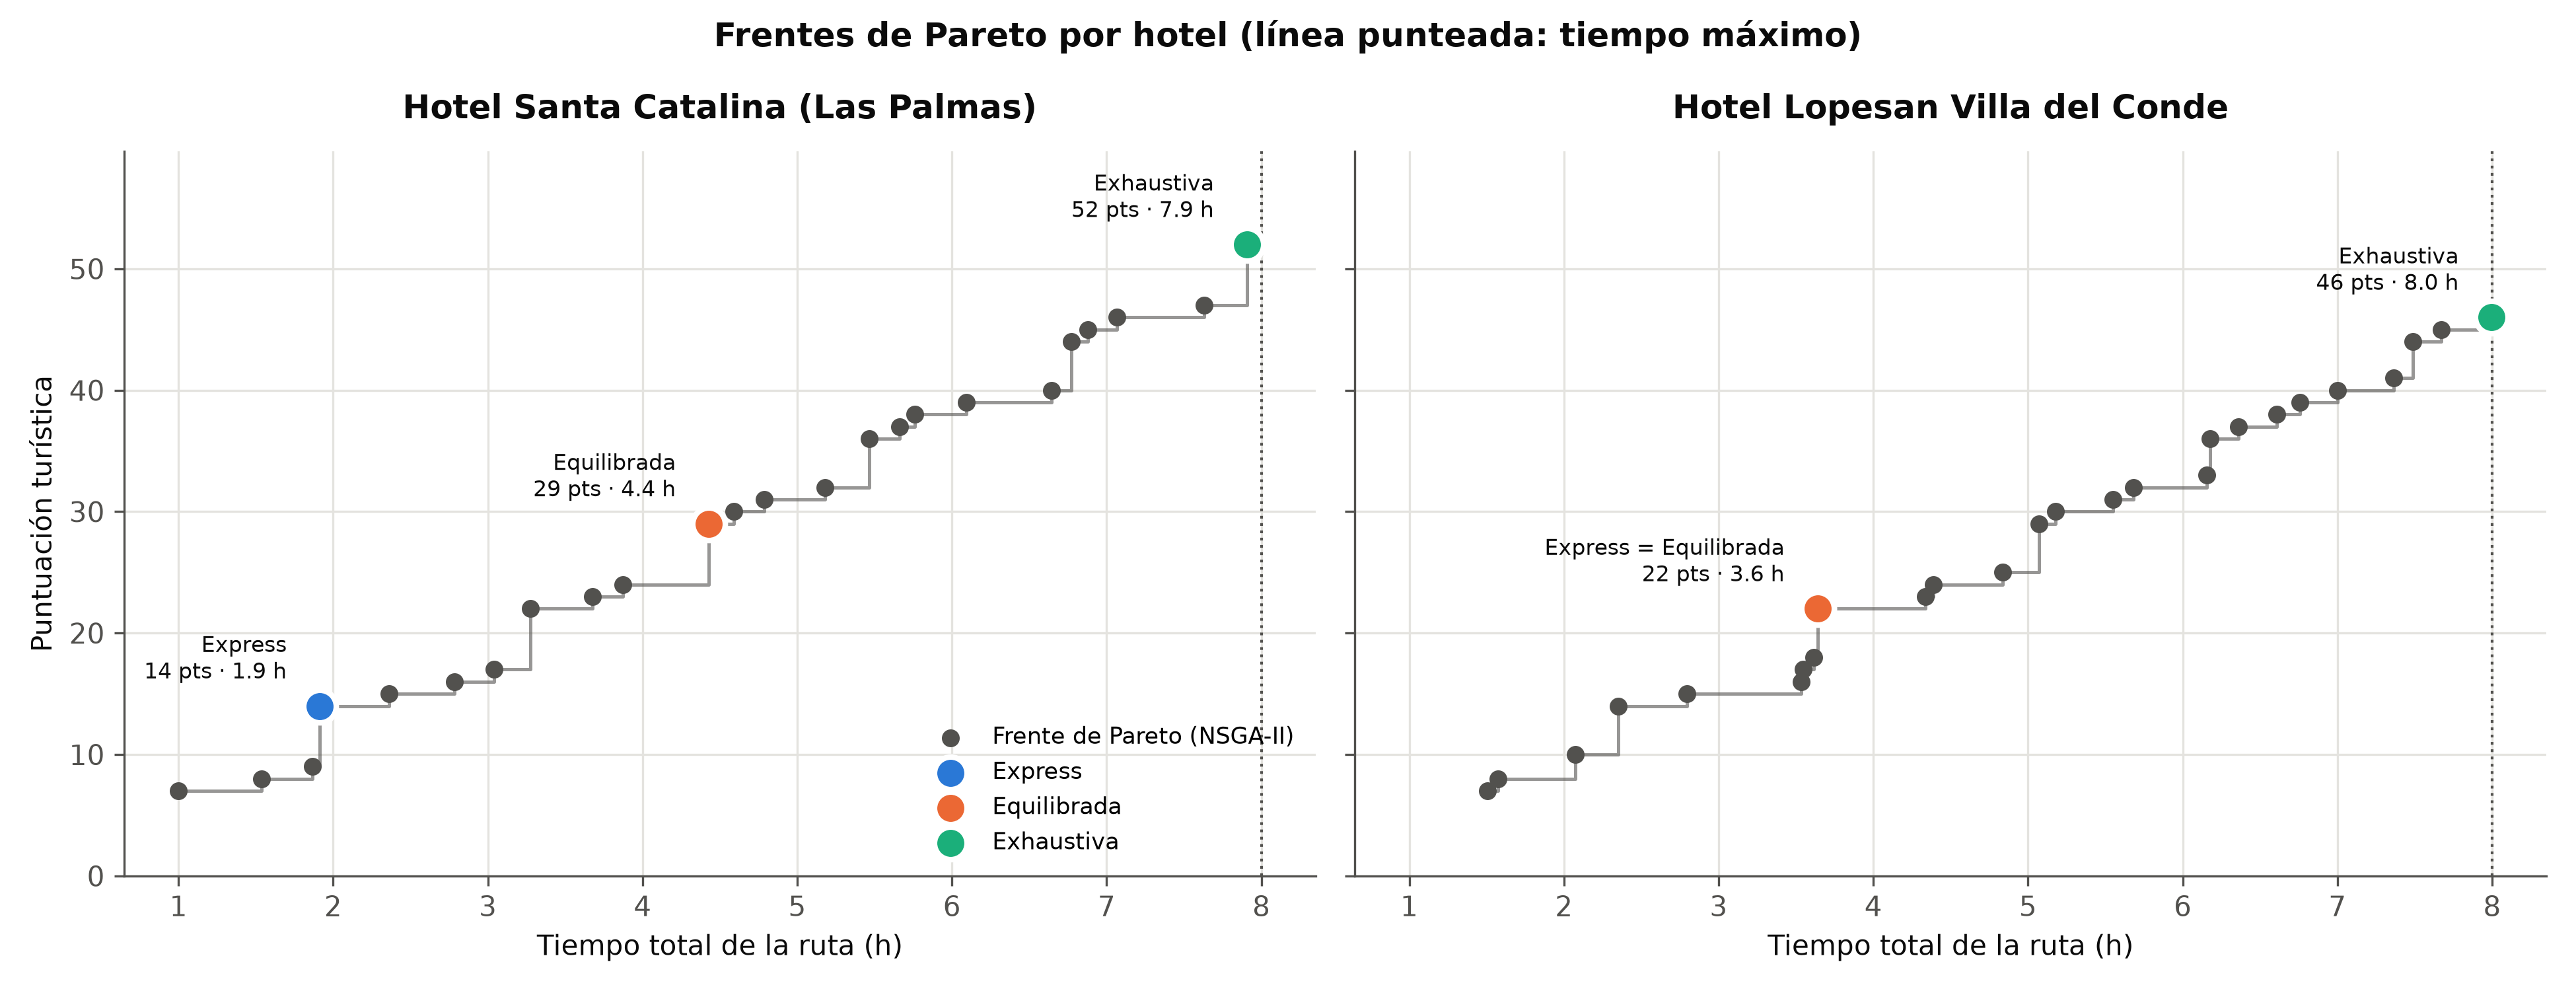
\includegraphics[width=\textwidth]{frentes_pareto.png}
\caption{Frentes de Pareto de cada hotel (semilla 42) con las rutas recomendadas. La línea punteada marca $\Tmax = 8$ h.}
\label{fig:frentes}
\end{figure}

\begin{table}[H]
\centering
\small
\caption{Rutas recomendadas (semilla 42).}
\label{tab:rutas}
\begin{tabularx}{\textwidth}{@{}l l c c X@{}}
\toprule
Hotel & Ruta & Puntos & Tiempo & Paradas \\
\midrule
Santa Catalina & Express & 14 & 1,9 h & Tufia, Bufadero de la Garita \\
 & Equilibrada & 29 & 4,4 h & Arucas, Firgas, Tufia, Bufadero \\
 & Exhaustiva & 52 & 7,9 h & Cueva Pintada, Cenobio de Valerón, Firgas, Jardín de la Marquesa, Arucas, Tufia, Bufadero \\
\midrule
Lopesan & Express y Equilibrada & 22 & 3,6 h & Tufia, Bufadero de la Garita, Barranco de Fataga \\
 & Exhaustiva & 46 & 8,0 h & Tufia, Bufadero, Cueva Pintada, Firgas, Arucas, Barranco de Fataga \\
\bottomrule
\end{tabularx}
\end{table}

Los frentes tienen unas 25 soluciones y forma escalonada: cada escalón corresponde a añadir o cambiar una parada. Desde Lopesan, la mejor ruta alcanza menos puntuación (46 frente a 52) y el hipervolumen medio es un 13,6 \% menor, porque la mayoría de los POIs están en el norte y en la cumbre. En Lopesan la ruta Express coincide con la Equilibrada: la de mejor puntuación por hora es también el punto rodilla.

\subsection{Estudio de hiperparámetros}
\label{sec:hiperparametros}

Para comprobar la configuración de la tabla~\ref{tab:parametros} se probaron, con las mismas 15 semillas y 20.100 evaluaciones:
\begin{itemize}
  \item cuatro combinaciones de población y generaciones: (50, 401), (100, 200), (150, 133) y (300, 66);
  \item una rejilla de cruce $p_c \in \{0{,}6;\ 0{,}85;\ 0{,}95\}$ por mutación $p_m \in \{0{,}15;\ 0{,}35;\ 0{,}55\}$ con $N = 100$ y $G = 200$.
\end{itemize}
Cada alternativa se compara con la configuración actual mediante el test de Wilcoxon. Como son 11 comparaciones por hotel, además del umbral 0,05 se considera el de Bonferroni, $0{,}05/11 \approx 0{,}0045$.

\begin{table}[H]
\centering
\small
\caption{Estudio de hiperparámetros: diferencia del hipervolumen medio respecto a la configuración actual ($N = 100$, $G = 200$, $p_c = 0{,}85$, $p_m = 0{,}35$) y $p$-valor de Wilcoxon.}
\label{tab:hiperparametros}
\begin{tabular}{@{}cccc rr rr@{}}
\toprule
& & & & \multicolumn{2}{c}{Santa Catalina} & \multicolumn{2}{c}{Lopesan} \\
\cmidrule(lr){5-6}\cmidrule(lr){7-8}
$N$ & $G$ & $p_c$ & $p_m$ & Dif. & $p$ & Dif. & $p$ \\
\midrule
50 & 401 & 0,85 & 0,35 & +0,03 \% & 0,733 & +0,05 \% & 0,454 \\
150 & 133 & 0,85 & 0,35 & $-$0,17 \% & 0,454 & +0,01 \% & 1,000 \\
300 & 66 & 0,85 & 0,35 & $-$0,20 \% & 0,010 & $-$0,25 \% & 0,095 \\
100 & 200 & 0,60 & 0,15 & $-$0,59 \% & $3{,}1\cdot10^{-4}$ & $-$1,00 \% & 0,010 \\
100 & 200 & 0,60 & 0,35 & $-$0,03 \% & 0,889 & $-$0,09 \% & 0,890 \\
100 & 200 & 0,60 & 0,55 & +0,09 \% & 0,041 & +0,20 \% & 0,359 \\
100 & 200 & 0,85 & 0,15 & $-$0,42 \% & 0,002 & $-$0,85 \% & 0,010 \\
100 & 200 & 0,85 & 0,55 & +0,11 \% & 0,158 & +0,34 \% & 0,073 \\
100 & 200 & 0,95 & 0,15 & $-$0,53 \% & $8{,}5\cdot10^{-4}$ & $-$0,77 \% & 0,008 \\
100 & 200 & 0,95 & 0,35 & $-$0,08 \% & 0,330 & +0,01 \% & 0,847 \\
100 & 200 & 0,95 & 0,55 & +0,06 \% & 0,530 & +0,24 \% & 0,303 \\
\bottomrule
\end{tabular}
\end{table}

Las diferencias van del $-1{,}00$ \% al $+0{,}34$ \%, de modo que la configuración elegida es razonable. El parámetro que más influye es la mutación: con $p_m = 0{,}15$ el hipervolumen baja en todos los casos, y en Santa Catalina esas caídas siguen siendo significativas con Bonferroni. Subir la mutación a 0,55 tiende a mejorar (la mayor media en los dos hoteles se obtiene con $p_c = 0{,}85$ y $p_m = 0{,}55$), pero sin significación; como la mejora se ha observado con las mismas semillas con las que se elige, habría que confirmarla con semillas nuevas antes de cambiar el valor. El cruce apenas influye. La combinación (300, 66) es la peor en los dos hoteles: con solo 66 generaciones el algoritmo no llega a converger.

\subsection{Análisis de sensibilidad}
\label{sec:sensibilidad}

Como las puntuaciones y los tiempos de visita son ilustrativos, se repitió NSGA-II (15 semillas) con cuatro variantes de los datos, manteniendo la matriz de conducción y el límite de 8 horas: visitas multiplicadas por 0,75 y por 0,5; puntuación uniforme (todos los POIs valen 8,03, la media), con la que solo cuenta el número de paradas; y puntuación cuadrática $s^2/10$, que mantiene el 10 y rebaja las puntuaciones medias, de modo que pesan más los lugares icónicos.

\begin{table}[H]
\centering
\small
\caption{Análisis de sensibilidad (medias de 15 semillas). El hipervolumen de las variantes de puntuación no es comparable con el de la base porque cambia la escala.}
\label{tab:sensibilidad}
\begin{tabular}{@{}l l r c c@{}}
\toprule
Hotel & Variante & Hipervolumen & Soluciones & Paradas (ruta más completa) \\
\midrule
Santa Catalina & Base & 11.594,3 & 24,6 & 6,9 \\
 & Visitas $\times 0{,}75$ & 14.329,8 & 30,2 & 8,0 \\
 & Visitas $\times 0{,}5$ & 18.815,0 & 43,8 & 10,0 \\
 & Uniforme & 12.166,5 & 6,3 & 6,3 \\
 & Cuadrática & 8.998,2 & 53,8 & 6,0 \\
\midrule
Lopesan & Base & 10.013,1 & 23,6 & 6,0 \\
 & Visitas $\times 0{,}75$ & 12.261,1 & 27,3 & 7,0 \\
 & Visitas $\times 0{,}5$ & 16.064,1 & 40,1 & 9,0 \\
 & Uniforme & 10.478,2 & 5,9 & 5,9 \\
 & Cuadrática & 7.941,0 & 25,1 & 5,2 \\
\bottomrule
\end{tabular}
\end{table}

Acortar las visitas a la mitad aumenta el hipervolumen un 62 \% en Santa Catalina y un 60 \% en Lopesan, y la ruta más completa pasa de 6--7 paradas a 9--10. Con puntuación uniforme el frente se reduce a unas 6 soluciones, una por número de paradas, porque entre dos rutas con las mismas paradas solo sobrevive la más corta.

Más revelador es qué POIs aparecen. En todas las variantes y en los dos hoteles, el Bufadero de la Garita, Tufia y Arucas forman el núcleo de las rutas: son visitas cortas en el noreste, junto a la autopista GC-1. En cambio, las Dunas de Maspalomas y el Roque Nublo, con la máxima puntuación, casi nunca aparecen. La tabla~\ref{tab:iconos} explica por qué: ir, visitarlos y volver cuesta más de tres horas por 10 puntos, mientras que la ruta Express de Santa Catalina da 14 puntos en 1,9 horas.

\begin{table}[H]
\centering
\small
\caption{Tiempo de ir, visitar y volver ($t_{hi} + v_i + t_{ih}$, en minutos) para los dos lugares de puntuación 10 menos elegidos.}
\label{tab:iconos}
\begin{tabular}{@{}l c c@{}}
\toprule
Desde & Dunas de Maspalomas & Roque Nublo \\
\midrule
Santa Catalina & $42{,}2 + 120 + 42{,}7 = 205{,}0$ & $69{,}2 + 90 + 70{,}8 = 230{,}0$ \\
Lopesan & $2{,}3 + 120 + 2{,}2 = 124{,}4$ & $56{,}3 + 90 + 55{,}5 = 201{,}8$ \\
\bottomrule
\end{tabular}
\end{table}

Desde Santa Catalina ninguno de los dos aparece en ninguna variante. Desde Lopesan las Dunas sí están en el 28,5 \% de las soluciones del frente, pero solo en rutas cortas, y entran en las rutas recomendadas en cuanto la visita se acorta o el 10 pesa más. El Roque Nublo solo gana presencia con la puntuación cuadrática (del 1,4 \% al 19,4 \% de las soluciones desde Lopesan); acortar la visita no basta, porque lo que pesa es la conducción de ida y vuelta, casi dos horas.
